\chapter{Introduction}
\label{cha:intro}
\subsection{Importance of topic}
"Society expects autonomous vehicles to be held to a higher standard than human drivers." \cite{Prof.Amnon} This quote is setting the tone of the technology in autonomous driving. In order to be accepted to the public, autonomous vehicles should perform as least as good as the conventional human driver on parameters as for example safety. Despite widespread research on self-driving vehicles the acceptance by the user stays only limited.\cite{Bae2019} The purchase behaviour of customers can be linked with a good feeling which is directly connected with comfort. Also in order to gain more trust by the public it is clear that the challenge of making autonomous vehicles as comfortable as possible, should be tackled. This immediately leads to the questions what comfort during driving exactly is and how to measure it.\\
Driving comfort is a personal experience and also depend on the current emotional state of the driver. This means that more than one driving style for autonomous vehicle-driving should be identified for a certain vehicle. \cite{Eindhoven2019} The state of the driver can be communicated with the vehicle at the start of the ride. 

\begin{figure}[h!]
	\centering
	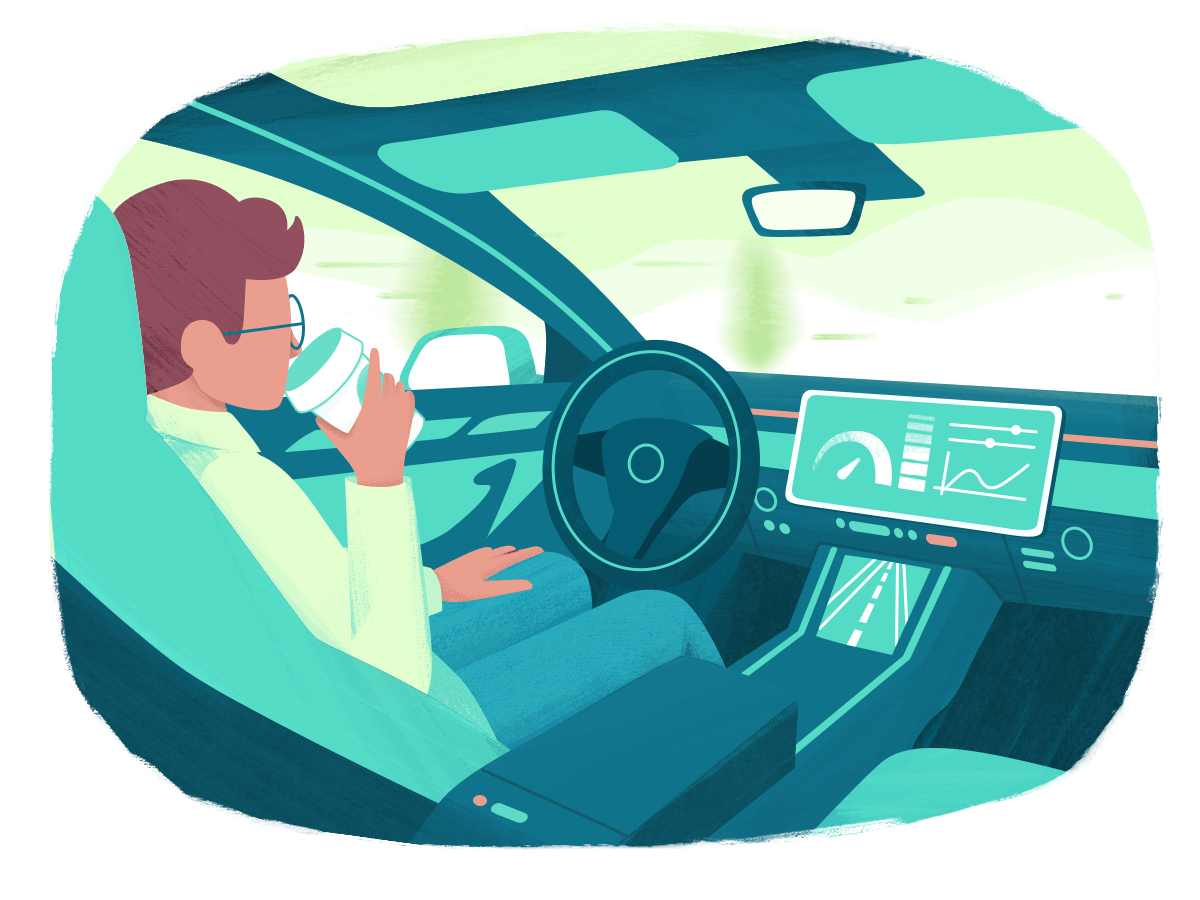
\includegraphics[width=0.6\linewidth]{AV}
	\caption{Concept visualization of autonomous driving. (source: \cite{AV})}
	\label{fig:AV}
\end{figure} 

\subsection{Link with previous studies and problem formulation}

In order to identify the specific comfort preferences of the driver, it should be able to learn them by demonstration. \cite{Kuderer2015a}\\
Despite that each driver has its own preferences, they are based on a common notion of comfort where only different trade-offs are made. For example some drivers prefer more aggressive driving behaviour than others which will manifests itself in a different trade off of different comfort criteria than for example a defensive drivers. This will later in this thesis be translated into a comfort objective where different weights are used in order to quantify different comfort trade-offs made. \\

In order to find comfort criteria which can be used to distinguish different drivers, research about the notion of comfort is necessary. Passenger surveys in public road transport about carsickness \cite{Turner1999} have revealed that lateral motions and non-smooth driving behaviour could be best correlated with car sickness. There is a consensus reached about the contribution of continuous trajectories to the prevention of motion sickness and the natural feel of paths.\cite{Elbanhawi2015} This means that higher order kinematic variables like accelerations and jerks also should be considered in the assessment of comfort.\\

\subsection{Thesis objective}
The goal of this thesis is to build further on the research of learning by demonstration which stayed with a theoretical idea. \cite{Kuderer2015a}.The investigation is mainly focussed on the practical implementation and validation of a learning algorithm that is able to capture user specific driving preferences in weights of a comfort objective function. The learning process is be done offline. The next step will be to cast this in a path planning MPC formulation which will be calculating online feasible and comfortable paths whereafter a there is looked at an MPC tracking algorithm to follow the planned path. \\

The execution of this research is conducted with the support of "Siemens Digital Industries Software - NVH R\&D engineering department" located in Leuven which made it possible to preserve the direct link with reality. Software was made available e.g. Simcenter Amesim and the possibility to validate the obtained algorithms with real driver data made it possible to make the results that could be obtained more significant.\\


\textit{Aanvullen
Bespreek de layout van de thesis die gebruikt werd --> check of wat verteld werd in de inleiding nog correct is. Wat is de kapstok?}


%\section{Wat moet er vermeld worden}
%(meer op het einde van de introductie)
%Dit hoofdstuk geeft vooral een overzicht over de theorie en de opbouw van het probleem.
%Wat zijn de doelen van het project --> zie slides / wat is de probleemstelling.
%Wat is de kapstok --> drie stappen learning, planning, controlling, validatie
%Hoe zal het er in grote lijnen uit gaan zien en welke softwares zijn er allemaal aan te pas gekomen
%Welke voorzieningen heeft Siemens hieromtrent.
%
%Wat is een optimal control problem en wat is model predictive control? (zie paper VS)
%--> wat dieper ingaan op wat ik geleerd heb bij het vak optimization --> zie ook important thesis notes van optimization
%
%Maak een overview van het control sequence --> flowchart zoals op p5 zwitser. Maak zo veel mogelijk om de stromingen van de stappen bijvoordbeeld 3 stappen in project goed weer te geven. Veel figuren!


%%% Local Variables: 
%%% mode: latex
%%% TeX-master: "thesis"
%%% End: 
